%% Requires compilation with XeLaTeX or LuaLaTeX
\documentclass[10pt,xcolor={table,dvipsnames},t]{beamer}
\usetheme{diapo}
\usepackage{amsmath}

\title[Lorenz]{Data assimilation for the Lorenz system}
\subtitle{Presentation (version 0)}
\author[name]{AYDOGDU Melissa, LECOURTIER Frédérique}
\institute{\large Strasbourg University}
\date{05 april 2022}

\useoutertheme{miniframes}

\begin{document}
	
	\begin{frame}
		\titlepage
	\end{frame}
	
	\AtBeginSection[]{
		\begin{frame}
			\vfill
			\centering
			\begin{beamercolorbox}[sep=5pt,shadow=true,rounded=true]{subtitle}
				\usebeamerfont{title}\insertsectionhead\par%
			\end{beamercolorbox}
			\vfill
		\end{frame}
	}



	\begin{frame}{Cemosis}
		
		\begin{minipage}{0.4\hsize}
			\pgfimage[width=\linewidth]{images/logo-cemosis.pdf}
		\end{minipage} \quad
		\begin{minipage}{0.5\hsize}
		Cemosis is hosted by the Institute of Advanced Mathematical Research (IRMA) and was created in January 2013. They use and develop toals in the fields of: 
			\begin{enumerate}[\textbullet]
				\item \textbf{MSO} \\
				Modeling Simulation and Optimization
				\item \textbf{DS} \\
				Data Science, Big Data, Smart Data
				\item \textbf{HPC} \\
				High Performance Computing, \\
				Parallel Computing, Cloud Computing
				\item \textbf{SI} \\
				Signal and Image processing
			\end{enumerate}
		\end{minipage}
	\end{frame}

	\begin{frame}{Objectives}
		
		 \begin{enumerate}[\textbullet]
			\item \textbf{para-real method} - \quad to accelerate the simulation of ODE
			\item \textbf{data assimilation}, especially
			\begin{itemize}
				\item understanding Kalman Filter
				\item understanding and using Ensemble Kalman Filter
			\end{itemize}
		\end{enumerate}	 	
		
	\end{frame}
	
	\begin{frame}{Roadmap}
		
		\pgfimage[height=5.5cm,width=11cm]{images/gantt}
	\end{frame}
	
	
	\begin{frame}[allowframebreaks]{Lorenz system}
		
		The system :
		$$\left\{\begin{aligned} 
			\frac{\partial x}{\partial t} &=\sigma(y(t)-x(t))\\
			\frac{\partial y}{\partial t}&=x(t)(r-z(t))-y(t) \\
			\frac{\partial z}{\partial t}&=x(t)y(t)-bz(t)
		\end{aligned}\right.$$
	
		where
		
		\begin{enumerate}[\textbullet]
			\item $\sigma > 0$  relates to the Prandtl number
			\item $r > 0$  relates to the Rayleigh
			\item $b > 0$ is a geometric factor
		\end{enumerate}
		
	\end{frame}
	
	
	\section{Numerical resolution with different methods}
	
	\begin{frame}{Methods used to solve Lorenz system}
		
		\begin{itemize}
			\item Discretization : \\
			\qquad 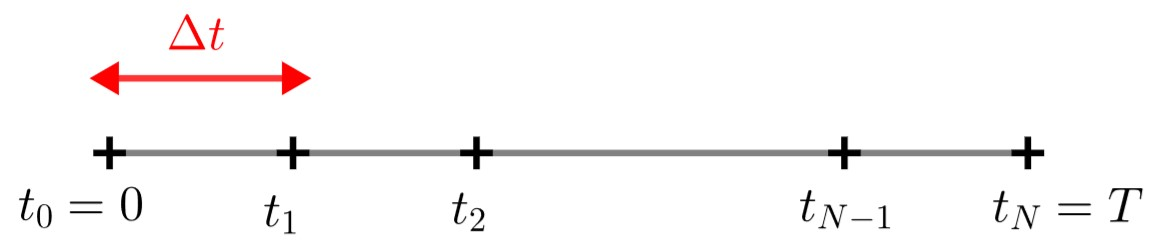
\includegraphics[width=0.4\textwidth]{images/discretization.jpg} \\
			\item Explicit Euler
			\item Implicit Euler			
			\item Runge Kutta order 4th			
			\item Scipy function : \qquad \textit{scipy.integrate.solve\_ivp}
		\end{itemize}
		
	\end{frame}
	
	\begin{frame}{Some results (with Python)}
		
		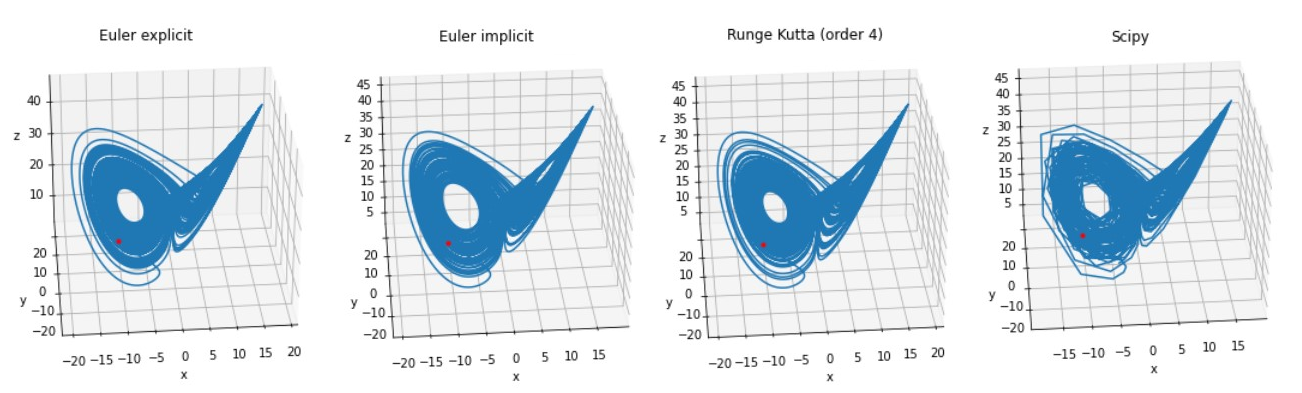
\includegraphics[width=\textwidth]{images/N100000.png} \\ 
		\begin{center}
			\begin{minipage}[c]{0.5\linewidth}
				$\sigma=10,\quad \beta=8/3, \quad r=28$ \\
				$X_0=(-10,10,5)$ 
			\end{minipage}
			$T=100, N = 100000 \Rightarrow \Delta t=0.001$
		\end{center}
		
	\end{frame}
	
\end{document}

